\documentclass{standalone}

\usepackage{tikz}
\usepackage{pgfplots}
\usepackage{amsmath}

\begin{document}
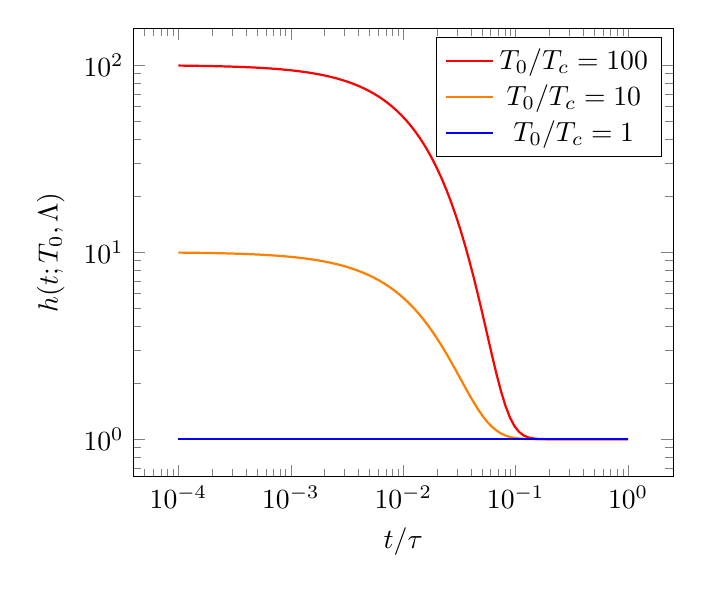
\begin{tikzpicture}
    \begin{loglogaxis}[ylabel={$h(t;T_0,\Lambda)$}, xlabel=$t/\tau$]
        \addplot[red, thick, domain=1e-4:1, samples=100]{(100-1)*exp(-65*x)+1};
        \addlegendentry{$T_0/T_c=100$};
        \addplot[orange, thick, domain=1e-4:1, samples=100]{(10-1)*exp(-65*x)+1};
        \addlegendentry{$T_0/T_c=10$};
        \addplot[blue, thick, domain=1e-4:1, samples=100]{(1-1)*exp(-65*x)+1};
        \addlegendentry{$T_0/T_c=1$};
    \end{loglogaxis}
\end{tikzpicture}
\end{document}